\documentclass[tikz,border=10pt]{standalone}
\usepackage{tikz}
\usetikzlibrary{calc}
\begin{document}
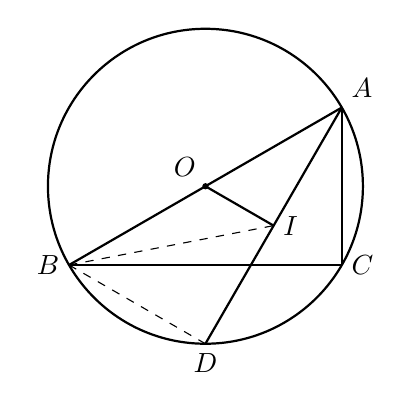
\begin{tikzpicture}[scale=2]
  % Draw the circle
  \draw[thick] (0,0) circle (1cm);
  
  % Define points on the circle
  \coordinate (O) at (0,0);
  \coordinate (A) at (0.866,0.5);
  \coordinate (B) at (-0.866,-0.5);
  \coordinate (C) at (0.866,-0.5);
  \coordinate (D) at (0,-1);
  
  % Define point I on segment AC
  \coordinate (I) at ($(A)!0.5!(D)$);
  
  % Draw the lines connecting points
  \draw[thick] (B) -- (A);
  \draw[thick] (B) -- (C);
  \draw[thick] (A) -- (C);
  \draw[thick] (A) -- (D);
  \draw[thick] (O) -- (I);
  \draw[dashed] (B) -- (I);
  \draw[dashed] (B) -- (D);
  
  % Draw and label points
  \fill (O) circle (0.02);
  \node[above left] at (O) {$O$};
  \node[above right] at (A) {$A$};
  \node[left] at (B) {$B$};
  \node[right] at (C) {$C$};
  \node[below] at (D) {$D$};
  \node[right] at (I) {$I$};
\end{tikzpicture}
\end{document}